\subsection{Propriedades Termofísicas}

Propriedades termofísicas – como massa específica, viscosidade, calor específico, condutividade térmica, entalpia e entropia – são insumos essenciais em praticamente todos os cálculos de processos. Em misturas, a predição de propriedades requer modelos mais complexos do que simples somas ponderadas, considerando interações moleculares e desvios da idealidade. Tais propriedades alimentam balanços de massa e energia, o dimensionamento térmico de trocadores, o cálculo de Reynolds e de fatores de atrito, o desempenho de separações, entre outros. Temperatura e pressão são variáveis determinantes: utilizam-se correlações empíricas (por exemplo, equação de Antoine para pressão de vapor) ou equações de estado (gás ideal, Peng-Robinson, SRK) conforme o sistema. Erros na estimativa de viscosidade ou massa específica afetam o cálculo de Reynolds, fator de atrito e potência de bombeamento; imprecisões em calores específicos ou entalpias propagam-se em balanços de energia e projeto de utilidades.

\begin{table}[H]
    \centering
    \caption{Fluxo de obtenção de propriedades termofísicas}
    \label{tab:fluxo-propriedades-termofisicas}
    \small
    \begin{tabular}{p{0.25\textwidth}p{0.57\textwidth}}
        \hline
        \textbf{Etapa} & \textbf{Descrição} \\
        \hline
        Entradas & Fluido, propriedade solicitada, temperatura em K e pressão em Pa; para propriedades críticas, apenas o fluido. \\
        Processamento & Consulta \textit{CoolProp}, trata propriedades de saturação e associa unidades SI por meio do \textit{Pint}. \\
        Saída & Propriedade solicitada ou conjunto de propriedades, incluindo propriedades críticas quando aplicável. \\
        Validação & Confere a existência do fluido e comunica falhas de consulta ou propriedades indisponíveis. \\
        \hline
    \end{tabular}
    \fonte{Autoria própria.}
\end{table}

No \textit{software} desenvolvido, um módulo de propriedades utiliza a biblioteca \textit{CoolProp} para recuperar propriedades de fluidos puros (e misturas) a partir de dados de entrada de $T$ e $P$. São obtidas propriedades como massa específica ($\rho$), viscosidade, calor específico ($c_{p}$ e $c_{v}$), condutividade térmica, entalpia, entropia, massa molar e tensão superficial, além de propriedades críticas e pontos de saturação (bolha/orvalho) quando aplicável. A visualização desse cálculo de propriedades, com foco no resultado para uma mistura, é apresentada na Figura \ref{fig:mixture_properties}.

\begin{figure}[H]
    \centering
    \caption{Interface de cálculo para as propriedades de uma mistura}
    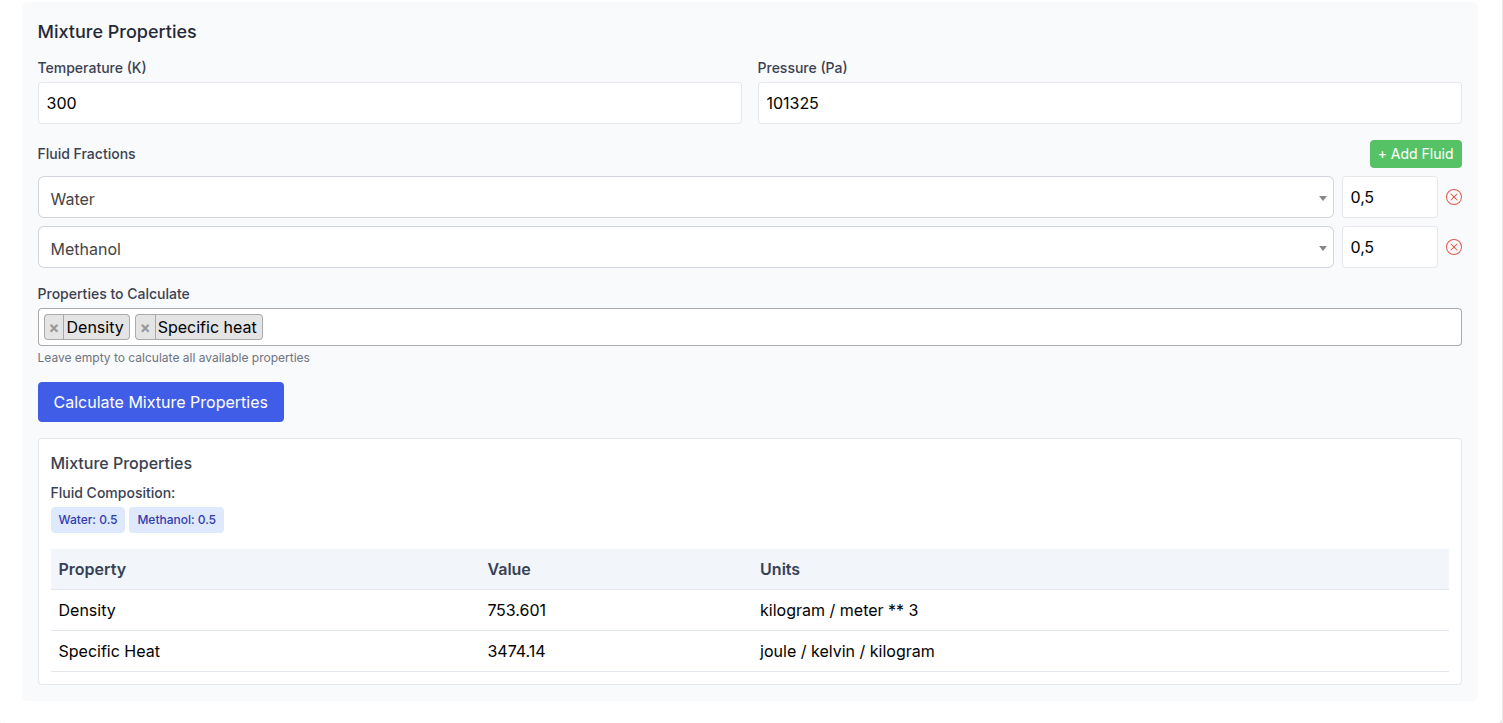
\includegraphics[width=\linewidth]{media/cap4_interface_propriedades_mistura.png}
    \fonte{Elaboração própria (2026).}
    \label{fig:mixture_properties}
\end{figure}

Para misturas, a \textit{API} do \textit{CoolProp} permite montar \textit{strings} com o padrão abaixo, usando as frações especificadas para cada componente \cite{bell2014}:

\begin{quote}
\small\texttt{HEOS::Comp1[x1]\&Comp2[x2]\&...}
\end{quote}

Todas as grandezas retornam já associadas a unidades do SI (via integração com a biblioteca \textit{Pint}), garantindo consistência nos cálculos.

\begin{table}[H]
    \centering
    \caption{Fluxo de obtenção de propriedades de misturas}
    \label{tab:fluxo-propriedades-misturas}
    \small
    \begin{tabular}{p{0.25\textwidth}p{0.57\textwidth}}
        \hline
        \textbf{Etapa} & \textbf{Descrição} \\
        \hline
        Entradas & Frações dos componentes, temperatura, pressão e, opcionalmente, a lista de propriedades. \\
        Preparação & Verifica os componentes, confere se as frações somam aproximadamente uma unidade e monta a representação da mistura. \\
        Processamento & Consulta as propriedades selecionadas na \textit{API} do \textit{CoolProp} usando a composição informada. \\
        Saída e validação & Retorna um conjunto de propriedades com unidades SI e rejeita componentes desconhecidos ou frações incompatíveis. \\
        \hline
    \end{tabular}
    \fonte{Autoria própria.}
\end{table}

O uso de uma biblioteca de propriedades de qualidade referência como o \textit{CoolProp} assegura que o \textit{software} tenha um \textit{backend} termodinâmico rigoroso e abrangente, reforçando o caráter didático ao permitir explorar diferentes cenários com fidelidade física.
